\subsection{Discharging Circuitry}

This section describes the operation of the discharging circuitry seen on Schematic Page: 4. It provides a means to determine the bulk capacitance value of the DUT from the RC time constant. Once the DUT is charged via the operation described in Section: \ref{sec:charging}, the charging relay will open and the high-current discharge relay will close. The transimpedance amplifier described in Section: \ref{sec:iMeas} will measure the current through the DUT as it decays.

There are 3 switched discharge stages that allow for the decay rate to be regulated. Each stage allows for a range of voltages and capacitances needed to stay within safety and operational constraints. As seen in Figure: \ref{fig:opArea}, there are two constraints on both the voltage and capacitance. The lowest valued resistor constrains the maximum voltage when using that stage due to its power rating. The other two stages are constrained by the overall safety limit of 500VDC. The minimum capacitance for each stage is determined by setting a requirement of at least $100$ ADC samples per time constant with a sampling rate of $250KSPS$. The maximum capacitance for each stage is determined by setting a maximum time constant.

\begin{figure}[ht!]
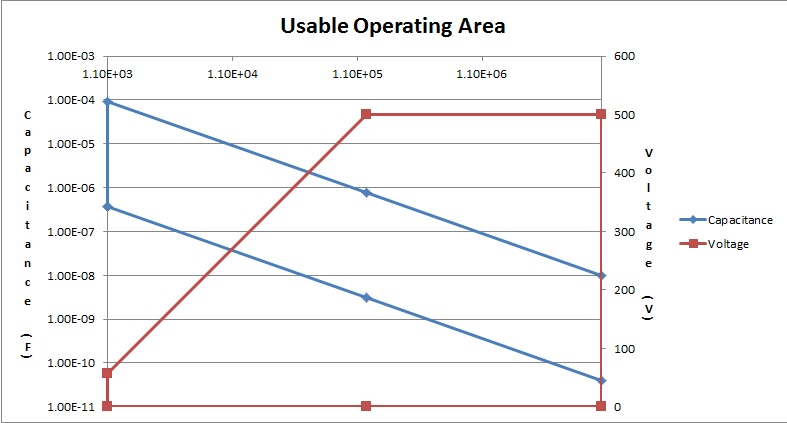
\includegraphics[keepaspectratio=true,width=3in]{./figures/circEx/operatingArea.jpg}
\centering
\caption{Operating Area}
\label{fig:opArea}
\end{figure}


The AD817 op-amp has the precision and bandwidth needed to operate in the transimpedance amplifier, but not the drive strength for th high current range. This limitation is overcome by inserting a BJT based current booster in the feedback path. This preserves the benefits of the op-amp, while providing the ability to drive a high-current signal.

